\documentclass[11pt, oneside]{article}   	% use "amsart" instead of "article" for AMSLaTeX format
\usepackage{geometry}                		% See geometry.pdf to learn the layout options. There are lots.
\geometry{letterpaper}                   		% ... or a4paper or a5paper or ... 
%\geometry{landscape}                		% Activate for for rotated page geometry
%\usepackage[parfill]{parskip}    		% Activate to begin paragraphs with an empty line rather than an indent
\usepackage{graphicx}				% Use pdf, png, jpg, or eps§ with pdflatex; use eps in DVI mode
								% TeX will automatically convert eps --> pdf in pdflatex		
\usepackage{amssymb}
\usepackage{amsmath}
\usepackage{parskip}
\usepackage{color}
\usepackage{hyperref}

\title{Binomial distribution}
%\author{The Author}
\date{}							% Activate to display a given date or no date

\graphicspath{{/Users/telliott_admin/Tex/png/}}
\usepackage{hyperref}

\begin{document}

\maketitle
%\section{}
%\subsection{}
\Large
You are likely familiar with the binomial distribution from algebra.  This distribution gives both the coefficients and the powers for each term in an expansion of the form
\[ (a+b)^n \]
where $n$ is a positive integer.  The first four examples are:
\[ (a+b)^1 = a + b \]
\[ (a+b)^2 = a^2 + 2ab + b^2 \]
\[ (a+b)^3 = a^3 + 3a^2b + 3ab^2 + b^3 \]
\[ (a+b)^4 = a^4 + 4a^3b + 6a^2b^2 + 4ab^3 + b^4 \]
and in general
\[ (a+b)^n = c_0a^n + c_1a^{n-1}b + c_2a^{n-2}b^2 + \dots + c_{n-1}ab^{n-1} + c_nb^n \]
where the sequence of coefficients $c_k$ is palindromic, and each of the $c_k$ (from $k \rightarrow n/2$) is in increasing order.

Ignoring the powers $a^{n-k}b^k$ for the moment, the coefficients are
\[ 1 \ \ 1 \]
\[ 1 \ \ 2 \ \ 1 \]
\[ 1 \ \ 3 \ \ 3 \ \ 1 \]
\[ 1 \ \ 4 \ \ 6 \ \ 4 \ \ 1 \]
As you know, this pattern is called Pascal's Triangle.  One striking thing about the triangle is that each value which is not on an edge can be formed by adding together the two values that lie directly above it.

The values running down the left and right sides are always $1$.

Another approach is that, rather than formatting as a triangle, some people just make vertical columns:

$1 \ \ 1$

$1 \ \ 2 \ \ 1$

$1 \ \ 3 \ \ 3 \ \ 1$

$1 \ \ 4 \ \ 6 \ \ 4 \ \ 1$

The first column contains only $1$'s, the second column is the natural numbers (or positive integers), and the third is the "triangular" numbers, where the difference between successive numbers is the sequence of natural numbers.

We will be very interested in the general case, and therefore we need to set a convention for going across a row $n$ using the index $k$.  Notice that the fourth row $n = 4$ has five terms.  It is convenient to let the index run from $k=0$ to $k = n$.

We can formalize the observation that a value is the sum of the two values above it by saying that the coefficient at position $k$ of row $n$ is the sum of the values at positions $k$ plus position $k-1$ of the preceeding row $n-1$.  For example, for $n=4$, the $k=2$ value is $6$.  $6$ is the sum of the values at $k=2$ and $k=1$ of the row for $n=3$.  Continuing:

$1 \ \ 4 \ \ 6 \ \ 4 \ \ 1$

$1 \ \ 5 \ 10 \ 10 \ 5 \ \ 1$

$1 \ \ 6 \ 15 \ 20 \ 15 \ \ 6 \ \ 1$

The corresponding expansions are:
\[ (a+b)^4 = a^4 + 4a^3b + 6a^2b^2 + 4ab^3 + b^4 \]
\[ (a+b)^5 = a^5 + 5a^4b + 10a^3b^2 + 10a^2b^3 + 5ab^4 + b^5 \]
\[ (a+b)^6 = a^6 + 6a^5b + 15a^4b^2 + 20a^3b^3 + 15a^2b^4 + 6ab^5 + b^6 \]

The power terms (leaving the coefficients out for the moment) are written in order as decreasing powers of $a$, starting from $n$, and increasing powers of $b$, starting from $0$:
\[ a^nb^0 + a^{n-1}b^1 + a^{n-2}b^2 + \dots + a^2b^{n-2} + ab^{n-1} + a^0b^n \]
which is the same as
\[ a^n + a^{n-1}b^1 + a^{n-2}b^2 + \dots + a^2b^{n-2} + ab^{n-1} + b^n \]

\subsection*{understanding the pattern}
In multiplying
\[ (a + b)(a + b) = a^2 + 2ab + b^2 \]
we can think of a generative procedure that goes term-by-term through the second multiplicand, multiplying first by $a$ on the left
\[ a \cdot (a + b) = a^2 + ab \]
and then by $b$ on the right
\[ (a + b) \cdot b = ab + b^2 \]
Finally, add the two results together:
\[ a \cdot (a + b) + (a + b) \cdot b \]
\[ = a^2 + ab + ab + b^2 \]
\[ = a^2 + 2ab + b^2 \]
We see that the two terms with the same power $a^1b^1$ come from multiplying $a \cdot (b)$ on the first pass, then adding $(a) \cdot b$ from the second.

This seems quite obvious, but it sets the stage for looking at a more complicated case.

In the expansion for $(a+b)^5$
\[ (a+b)^5 = a^5 + 5a^4b + 10a^3b^2 + 10a^2b^3 + 5ab^4 + b^5 \]
the coefficient of the $n=5$, $k=2$ term $a^3b^2$ is $10$.  We can get that $10$ by taking two terms from the expansion for $(a+b)^4$
\[ (a+b)^4 = a^4 + 4a^3b + 6a^2b^2 + 4ab^3 + b^4 \]

Namely, the $n=4$, $k = 2$ term is multiplied by $b$
\[ (4a^3b) \cdot b \]
and the $n=4$, $k=3$ term is multiplied by $a$
\[ a \cdot (6a^2b^2)  \]
when the two results are added together we obtain
\[ (4a^3b) \cdot b + a \cdot (6a^2b^2) = 10a^3b^2 \]

For the general case, we see that in writing the expansion for row $n+1$, at the $k$th term we form the power
\[ a^{n+1-k}b^{k} \] 

We have two contributions from the previous row.  One comes from multiplying
\[ a^{n+1-k}b^{k-1} \cdot b \]
and the second comes from
\[ a \cdot a^{n-k}b^{k} \]

The term that is multiplied by $a$, namely $a^{n-k}b^{k}$, is found at the same column, immediately above $a^{n+1-k}b^{k}$.

The other one, $a^{n-k+1}b^{k-1}$ (the same as $a^{n+1-k}b^{k-1}$), is the term that precedes it.  (Recall that powers of $a$ get larger as we go to the left, and powers of $b$ get smaller).

This explains why we obtain the pattern seen in Pascal's triangle as the coefficients for each expansion.  As we said before:  the coefficient at the position $k$ of row $n$ is the sum of the values at positions $k$ and $k-1$ of row $n-1$.

\subsection*{choose}
There is a very useful formula that allows one to find the coefficients of each term in the binomial expansion without actually filling out the triangle.  It is called "n choose k".

The official way to write this expression is
\[  {{n}\choose{k}} \]

The formula is: 
\[  {{n}\choose{k}} = \frac{n!}{(n-k!) \ k!} \]

This gives the number of different combinations of $k$ objects one can choose from $n$ total objects.  For example, suppose you have 5 Bob Marley CD's, and you want to pick 2 of them to take to a party, that is "5 choose 2" and the formula is
\[ \frac{5!}{3! \ 2!} = \frac{5 \times 4 \times 3 \times 2 }{3 \times 2 \times 2} = \frac{120}{12} = 10 \]

This is also the coefficient in row $n$, position $k$ of Pascal's Triangle (indexing from $k=0$).  

For our example, that is row $5$ position $2$.

$1 \ \ 5 \ 10 \ 10 \ 5 \ \ 1$

\[ (a+b)^5 = a^5 + 5a^4b + 10a^3b^2 + 10a^2b^3 + 5ab^4 + b^5 \]
which is indeed 10.

Notice a cancellation we can do in our formula.  We we rewrite the numerator with $n!$:
\[ \frac{n \times (n-1) \cdots \times (n-k+1) \times (n-k)! \cdots}{(n-k)! \ k!}  \]

We can cancel the factor of $(n-k)!$ and then have
\[ \frac{n(n-1) \cdots (n-k+1)}{k!} \]
In the example:
\[ \frac{5 \times 4 \times 3 \times 2 }{3 \times 2 \times 2} = \frac{5 \times 4 }{2} = \frac{20}{2} = 10 \]
It is a good idea to memorize the combinations formula.  It comes up repeatedly, in the derivations of calculus, and in probability.  

\subsection*{quick derivation of the choose formula}
Suppose you have $n$ CD's and you want to pick 2 of them to take with you.  There are $n$ choices for the first one---maybe you choose \emph{Natty Dread}.  And there are $n-1$ choices for the second one, you pick \emph{Kaya}.

That would give $n \cdot (n-1)$ here, and in the general case $n \cdot (n-1) \cdot \dots (n-k+1)$.  However, the order is not important, you might just as well have picked \emph{Kaya} and then \emph{Natty Dread}.  That's why we have to correct for the over-counting.  In this particular case we divide by $2$, and in the general case divide by k!.

\subsection*{Binomial theorem:  proof}
A concise statement of the binomial formula is that the general term is of the form
\[ {{n}\choose{k}} \ a^{n-k} \ b^k  \]
and the whole sum is
\[ \sum_{k=0}^{n} {{n}\choose{k}} \ a^{n-k} \ b^k  \]

where (from the theory of combinations):
\[  {{n}\choose{k}} = \frac{n!}{(n-k)! \ k!} \]
To do an actual calculation, we would first cancel the factor of $(n-k)!$ on top and bottom yielding
\[  {{n}\choose{k}} = \frac{n \times (n-1) \dots \times (n-k+1)}{k!} \]

\subsection*{Pascal's Lemma}
In order to prove the theorem (using induction) we will need the following result:

\[  {{n}\choose{k}} = {{n-1}\choose{k}} + {{n-1}\choose{k-1}} \]

Here is a simple proof of this result, from the theory of combinations.  Imagine that we are considering how many ways there are of forming a committee of $k$ members from a total of $n$ people.

We know that the number of ways of doing this is of course just
\[  {{n}\choose{k}} \]

Now, suppose that among these $n$ people we focus on one particular person, call her Alice.  Then there are two types of committees in our collection of combinations:  those in which Alice is a member, and those in which she is not.

For all committees of the first type, in addition to Alice, the other $k-1$ members must be drawn from $n-1$ people. The number of ways of doing this is
\[  {{n-1}\choose{k-1}} \]

For the second case, where Alice is not a member, we must recruit all $k$ members from $n-1$ people, since we are leaving Alice out.  The number of ways of doing this is
\[  {{n-1}\choose{k}} \]

But putting them together, these must be equal to the total number obtained by the standard analysis, and hence we have that
\[  {{n}\choose{k}} = {{n-1}\choose{k}} + {{n-1}\choose{k-1}} \]

This is effectively what we said near the beginning of the introduction to the binomial theorem:  in computing the $k$th coefficient in the $n$th row, we add the $k$ and $k-1$ values from the preceding row.

This preliminary result is called Pascal's Lemma and it is really the heart of the proof.

In using it below, we will alter its form slightly by substituting $n+1$ for $n$.  Thus:
\[  {{n+1}\choose{k}} = {{n}\choose{k}} + {{n}\choose{k-1}} \]

\subsection*{Induction}

If we look at one more term in the expansion for $(a+b)^n$, writing the term preceding the one given above, we have
\[ (a+b)^n = \dots + {{n}\choose{k-1}} \ a^{n-k+1} \ b^{k-1} + {{n}\choose{k}} \ a^{n-k} \ b^k + \dots  \]
Notice that the exponent decreases by one for $a$ as we move to the right, while it increases by one for $b$.

When we form the new general term in the expansion for $(a+b)^{n+1}$, as we said before, we multiply the first term by $b$ and the second one by $a$, obtaining
\[ \dots + b {{n}\choose{k-1}} \ a^{n-k+1} \ b^{k-1} + a {{n}\choose{k}} \ a^{n-k} \ b^k + \dots  \]
\[ = \dots +  {{n}\choose{k-1}} \ a^{n-k+1} \ b^{k} + {{n}\choose{k}} \ a^{n-k + 1} \ b^k + \dots  \]
But these two powers are the same, and since
\[ n-k+1 = (n + 1) - k \]
their sum is the general term in the expansion for $(a+b)^{n+1}$
\[ = \dots + C \ a^{(n+1)-k} \ b^k + \dots  \]

In adding them, we add their coefficients:
\[  \dots +  \ [ \ {{n}\choose{k-1}} + {{n}\choose{k}} \ ] \  a^{(n+1)-k} \ b^{k} + \dots  \]

Referring back to Pascal's Lemma, we substitute
\[  {{n+1}\choose{k}} = {{n}\choose{k}} + {{n}\choose{k-1}} \]
yielding
\[  \dots +  \ {{n+1}\choose{k}} + a^{(n+1)-k} \ b^{k} + \dots  \]

We obtain the general term for the $n+1$ expansion.  This completes the inductive part of the proof.  It remains to check the binomial formula for a base case like $n=1$ or $n=2$, which I invite you to do.

$\square$

\subsection*{Courant's proof}
Courant gives a proof by induction which I've transcribed and annotated separately.  It duplicates significant parts of what we've already gone through, but there is some new material, which I've added in here.

Pascal's Lemma 
\[  {{n+1}\choose{k}} = {{n}\choose{k}} + {{n}\choose{k-1}} \]

was "proved" above by an argument about combinations which do or do not include a person named Alice.  In Courant's version, the factorials are manipulated to provide a direct mathematical proof.  

\subsection*{simplification}
As we saw before, in the choose formula, there are terms that cancel.  We expand $n!$ partially
\[ n! = n \cdot (n-1) \dots (n-k+1) \cdot (n-k)! \]
The last term is also present in the denominator of our formula
\[ C(n,k) = \frac{n!}{k! \ (n-k)!} \]
so we can simplify 
\[ C(n,k) = \frac{n \cdot (n-1) \dots (n-k+1)}{k!} \]

We will be interested in coefficients with $k+1$, so let's take a look at $n$ "choose" $k+1$.  The original definition would give:
\[ C(n,k+1) = \frac{n!}{(k+1)! \ (n-(k+1))!}  \]
Remove one set of parentheses
\[ = \frac{n!}{(k+1)! \ (n-k-1)!}  \]
By the same argument, expand $n!$
\[ = \frac{n \cdot (n-1) \dots (n-k+1) \cdot (n-k) \cdot (n-k-1)!}{(k+1)! \ (n-k-1)!}  \]
\[ = \frac{n \cdot (n-1) \dots (n-k+1) \cdot (n-k)}{(k+1)!} \]
You should convince yourself that the last term in the numerator is correct.  It seems somewhat counterintuitive that for $k+1$ the last term is $(n-k)$ rather than say, $(n-k+2)$, as I thought at first.

\subsection*{induction}
Let us examine the general statement
\[ C(n,k) + C(n,k+1) \]
Rewriting it as the factorial using the simplification we found above
\[ \frac{n \cdot (n-1) \dots (n-k+1)}{k!} + \frac{n \cdot (n-1) \dots (n-k+1) \cdot (n-k)}{(k+1)!} \]
We can factor out $(n-k)/(k+1)$ from the second term:
\[ = (\frac{n-k}{k+1}) \ \cdot \frac{n \cdot (n-1) \dots \ (n-k+1) }{k!}  \]
and we see that the second term is that factor multiplied by the first term.

Hence, the complete sum becomes
\[ \ [ \ 1 + (\frac{n-k}{k+1})  \ ] \  \cdot \frac{n \cdot (n-1) \dots \ (n-k+1) }{k!}  \]
Take the leading factor and put it over a common denominator
\[ \frac{(k+1) + (n-k)}{k+1} = \frac{n+1}{k+1} \]
so the expression now becomes
\[ = ( \frac{n+1}{k+1} ) \  \cdot \frac{n \cdot (n-1) \dots \ (n-k+1) }{k!}  \]
\[ = \frac{(n+1) \cdot n \cdot (n-1) \dots \ (n-k+1) }{(k+1)!}  \]
rearranging the last term in the numerator slightly
\[ = \frac{(n+1) \cdot n \cdot (n-1) \dots \ [ \ (n+1)-k \ ] }{(k+1)!}  \]
\[ = C(n+1,k+1) \]
This is the correct expression for $n+1$ (because it has $n+1$ in the right places), and it is the correct expression for $k+1$ because it ends with $n+1$ minus $k$ (rather than $k+1$).  

\subsection*{recap}
We assume that $C(n,k)$ is the correct coefficient for $a^{n-k}b^k$ in the expansion of $(a+b)^n$, and that $C(n,k+1)$ is the correct coefficient for the succeeding term $a^{n-(k+1)}b^{k+1}$ in the same expansion.  Multiplication of the first by $b$ and the second by $a$ leads to:
\[ \ [ \ C(n,k) + C(n,k+1) \ ] \ a^{n-k}b^{k+1} \]
We need to tweak one exponent slightly when considering this as part of the  expansion for $(a+b)^{n+1}$.  The $n$ in the exponent for $a$ should be expressed in terms of $n$ referring to the incremented value $n+1$ so it needs to step down one unit, becoming $a^{n-k - 1}$ which is equal to $a^{n-(k+1)}$ .  Thus we have
\[ \ [ \ C(n,k) + C(n,k+1) \ ] \ a^{n-(k+1)}b^{k+1} \]
We showed that 
\[ C(n,k) + C(n,k+1) = (1 + \frac{n-k}{k+1}) \cdot  C(n,k) \]
\[ = \frac{n+1}{k+1}) \cdot  C(n,k) \]
\[ = C(n+1,k+1) \]
which is what the binomial theorem gives.  This completes the proof by induction.
$\square$

\subsection*{probability}
The binomial theorem is also used extensively in working with discrete probability.  

A simple example is to consider a standard (6-sided), fair die.  We ask: 

What is the probability that in rolling six such dice (or one die six times), we will observe some distribution of results, like one or more 6's?

There is an easy way to do this.  We calculate the probability that no 6 is observed on one roll as 5/6 and on six rolls as

\[ (5/6)^6 = 15625/46656 = 0.334898 \]

The outcome of at least one 6 is the complement of this so its probability is $0.665102$.

The other way to do it is to use the formula that gives the distribution over all possible outcomes:

\[ C(n,k) p^k (1-p)^{n-k} \]

In this case, we have 
\large
\begin{verbatim}
C(6,0) = 1
C(6,1) = 6!/(1! 5!) = 6
C(6,2) = 6!/(2! 4!) = 15
C(6,3) = 6!/(3! 3!) = 720/36 = 20
C(6,4) = 15
C(6,5) = 6
C(6,6) = 1

P(0 6's) = 1          (5/6)^6 = 0.334898
P(1 6's) = 6  (1/6)   (5/6)^5 = 0.401878
P(2 6's) = 15 (1/6)^2 (5/6)^4 = 0.200939
P(3 6's) = 20 (1/6)^3 (5/6)^3 = 0.053584
P(4 6's) = 15 (1/6)^4 (5/6)^2 = 0.008038
P(5 6's) = 6  (1/6)^5 (5/6)^1 = 0.000643
P(6 6's) = 1  (1/6)^6         = 0.000021
\end{verbatim}
\Large
The total is $1.000001$, or 1, within the error introduced by truncation.

Suppose instead that we flip a (fair) coin 100 times.  What will be the distribution then? Since p = 1 - p = 0.5, the power terms are all the same, namely

\[ 0.5^{100} = 7.8886e-31 \]

But the factorials are kind of awkward.  For example, what is

\[ 100! / 50! 50! = ? \]

100! has 158 digits in it.  Python can do this calculation, the result is $1.008913e+29$ so we end up with $P = 0.0796$.

We use Python to compute the factorials in an efficient way, and tabulate the values for the probability from 35-50

\large
\begin{verbatim}
35 0.000863855665742
36 0.00155973939648
37 0.00269792760472
38 0.00447287997624
39 0.00711073226993
40 0.0108438667116
41 0.0158690732365
42 0.0222922695466
43 0.0300686426442
44 0.0389525597891
45 0.0484742966264
46 0.0579583981403
47 0.066590499991
48 0.0735270104067
49 0.0780286641051
50 0.0795892373872
\end{verbatim}
\Large
The distribution is symmetrical about the midpoint.

Adding up values gives the result that $99.8\%$ of the total probability lies between 35-65 inclusive.

Here is a plot of the values from 30-70.
\begin{center} 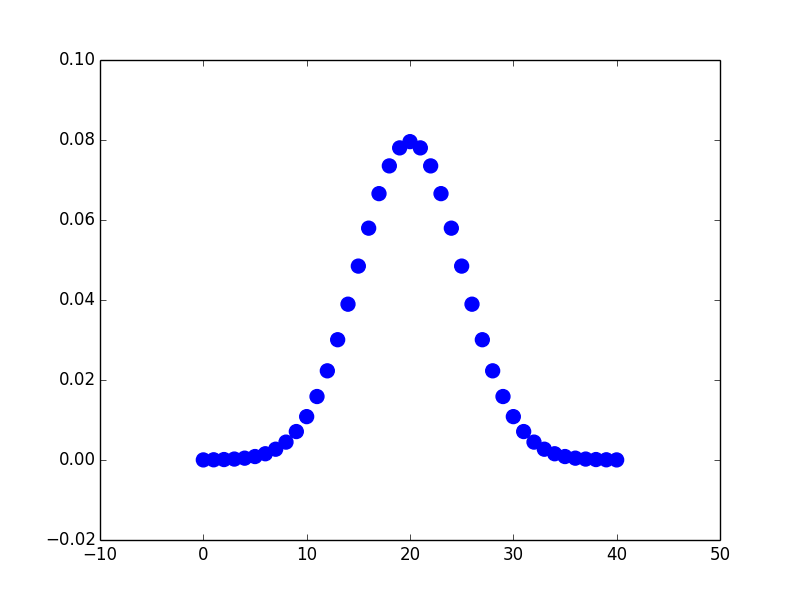
\includegraphics [scale=0.5] {binomial2.png} \end{center}
Look familiar?

\end{document}  